Antes de analizar los resultados, es importante precisar la metodología utilizada para la medición de memoria. 
En este trabajo, se consideró únicamente el peak de memoria dinámica (heap) utilizado por cada algoritmo. 
Es decir, no se incluyó el uso de memoria en el stack, ya que este corresponde a un consumo inevitable para cualquier algoritmo 
de ordenamiento o de multiplicación, siendo al menos proporcional al tamaño del arreglo o estructura de datos utilizada. 
Por esta razón, se decidió excluirlo del análisis.
En el caso de sort, el algoritmo ordena el arreglo in-place, por lo que no debería requerir memoria dinámica adicional. 
Sin embargo, en las mediciones realizadas se observó consistentemente un uso de memoria heap equivalente a 4n bytes, es decir, 
exactamente el tamaño de un arreglo de n enteros. Además, al modificar la función para que no retornara el vector y fuera de tipo void, 
dicha memoria adicional desapareció. Esto indica que el consumo registrado no proviene del algoritmo sort en sí, 
sino de la copia asociada al valor de retorno de la función utilizada en la implementación experimental. 
Por esta razón, dicha memoria fue descontada del análisis, sin modificar la implementación original entregada en el enunciado de la tarea.
\\
A continuación, se presenta el análisis de los algoritmos de ordenamiento de arreglos. 
En particular, se examinan las gráficas obtenidas a partir de los experimentos, con el objetivo de analizar 
el comportamiento temporal y de memoria de cada algoritmo de manera individual.
\begin{figure}[H]
    \centering
    \resizebox{\textwidth}{!}{
        \begin{minipage}{\textwidth}
            \centering

            \begin{subfigure}{0.48\textwidth}
                \centering
                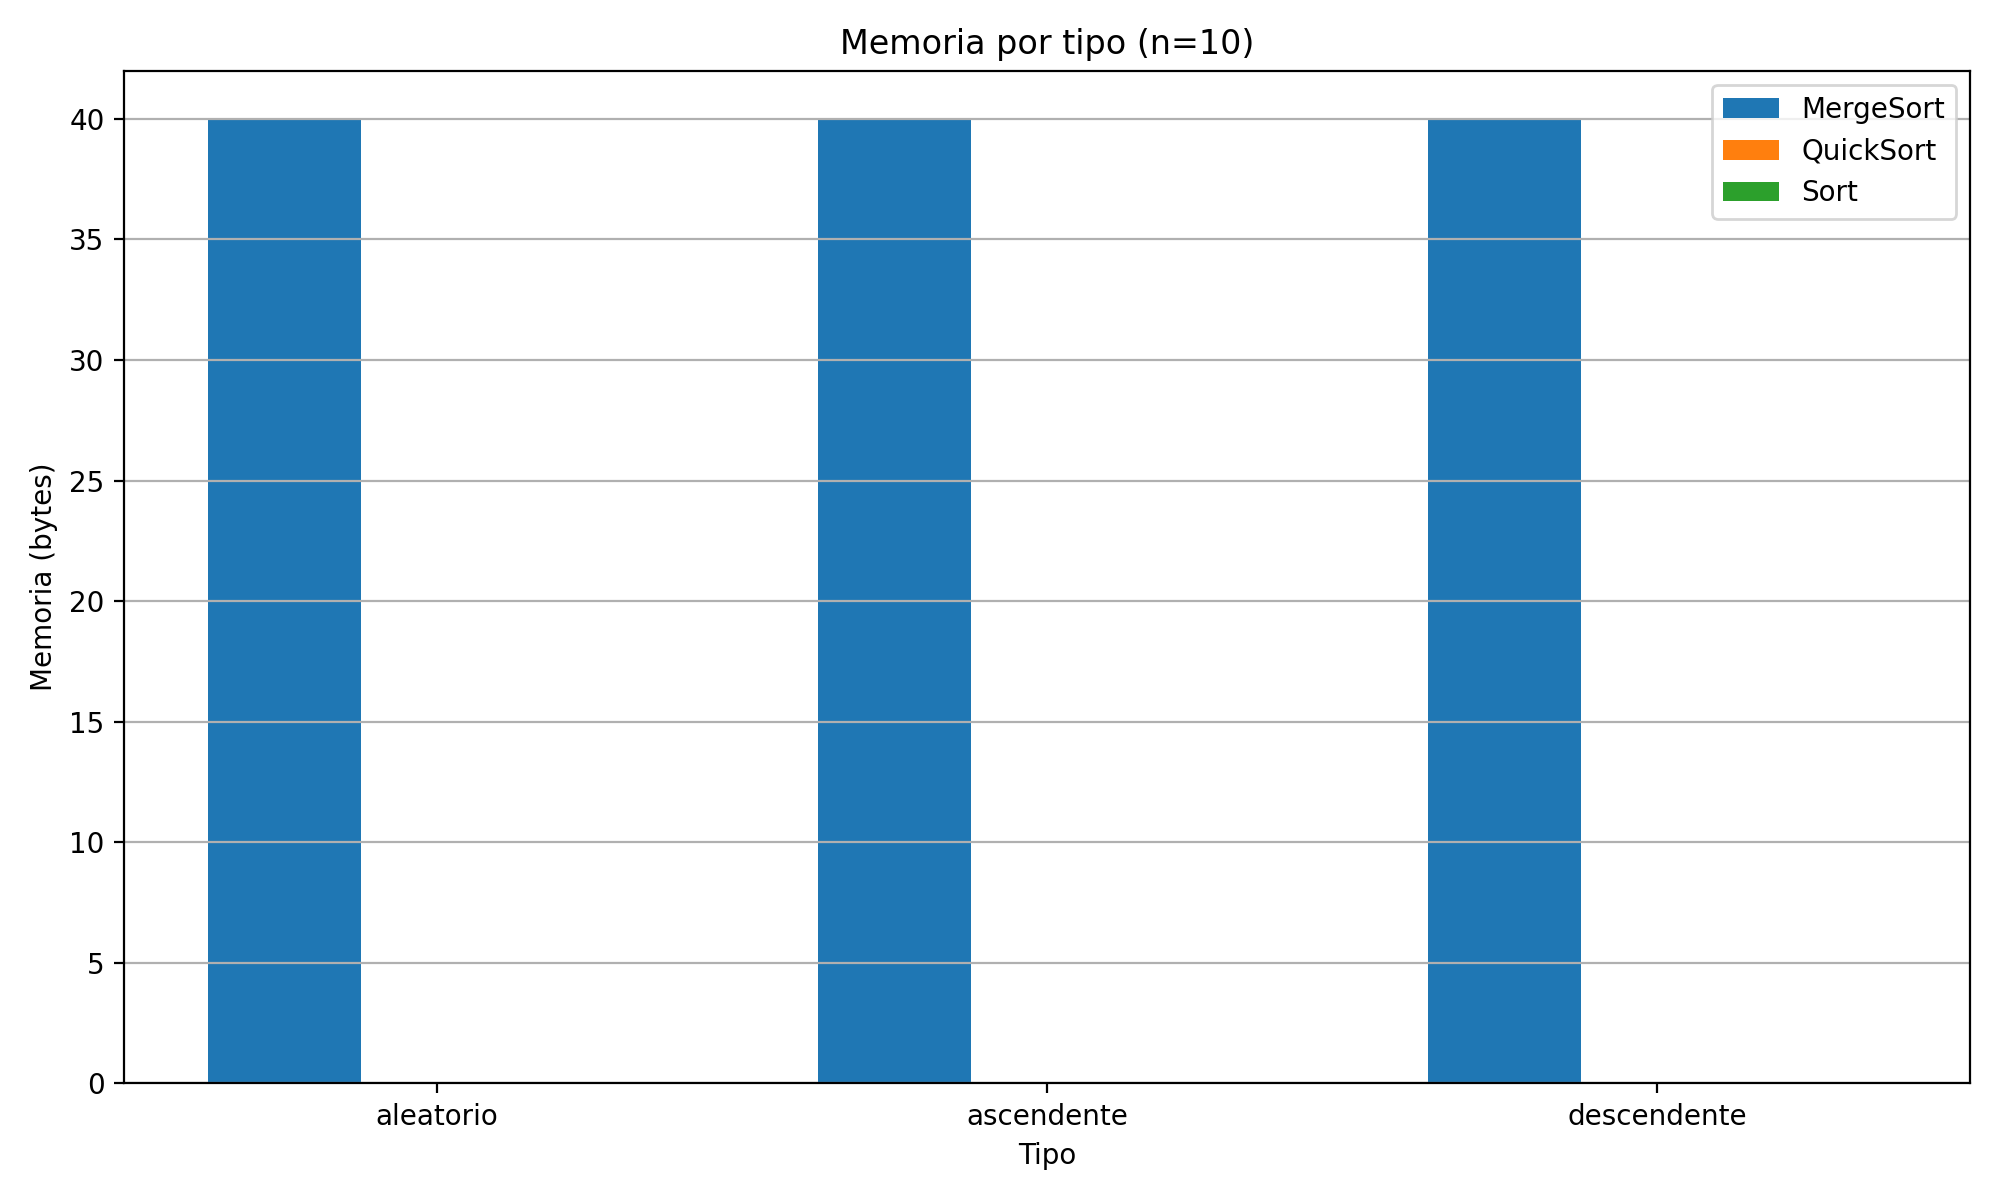
\includegraphics[width=\linewidth]{../code/sorting/data/plots/memory_n10.png}
                \caption{Memoria}
                \label{fig:img1}
            \end{subfigure}
            \hfill
            \begin{subfigure}{0.48\textwidth}
                \centering
                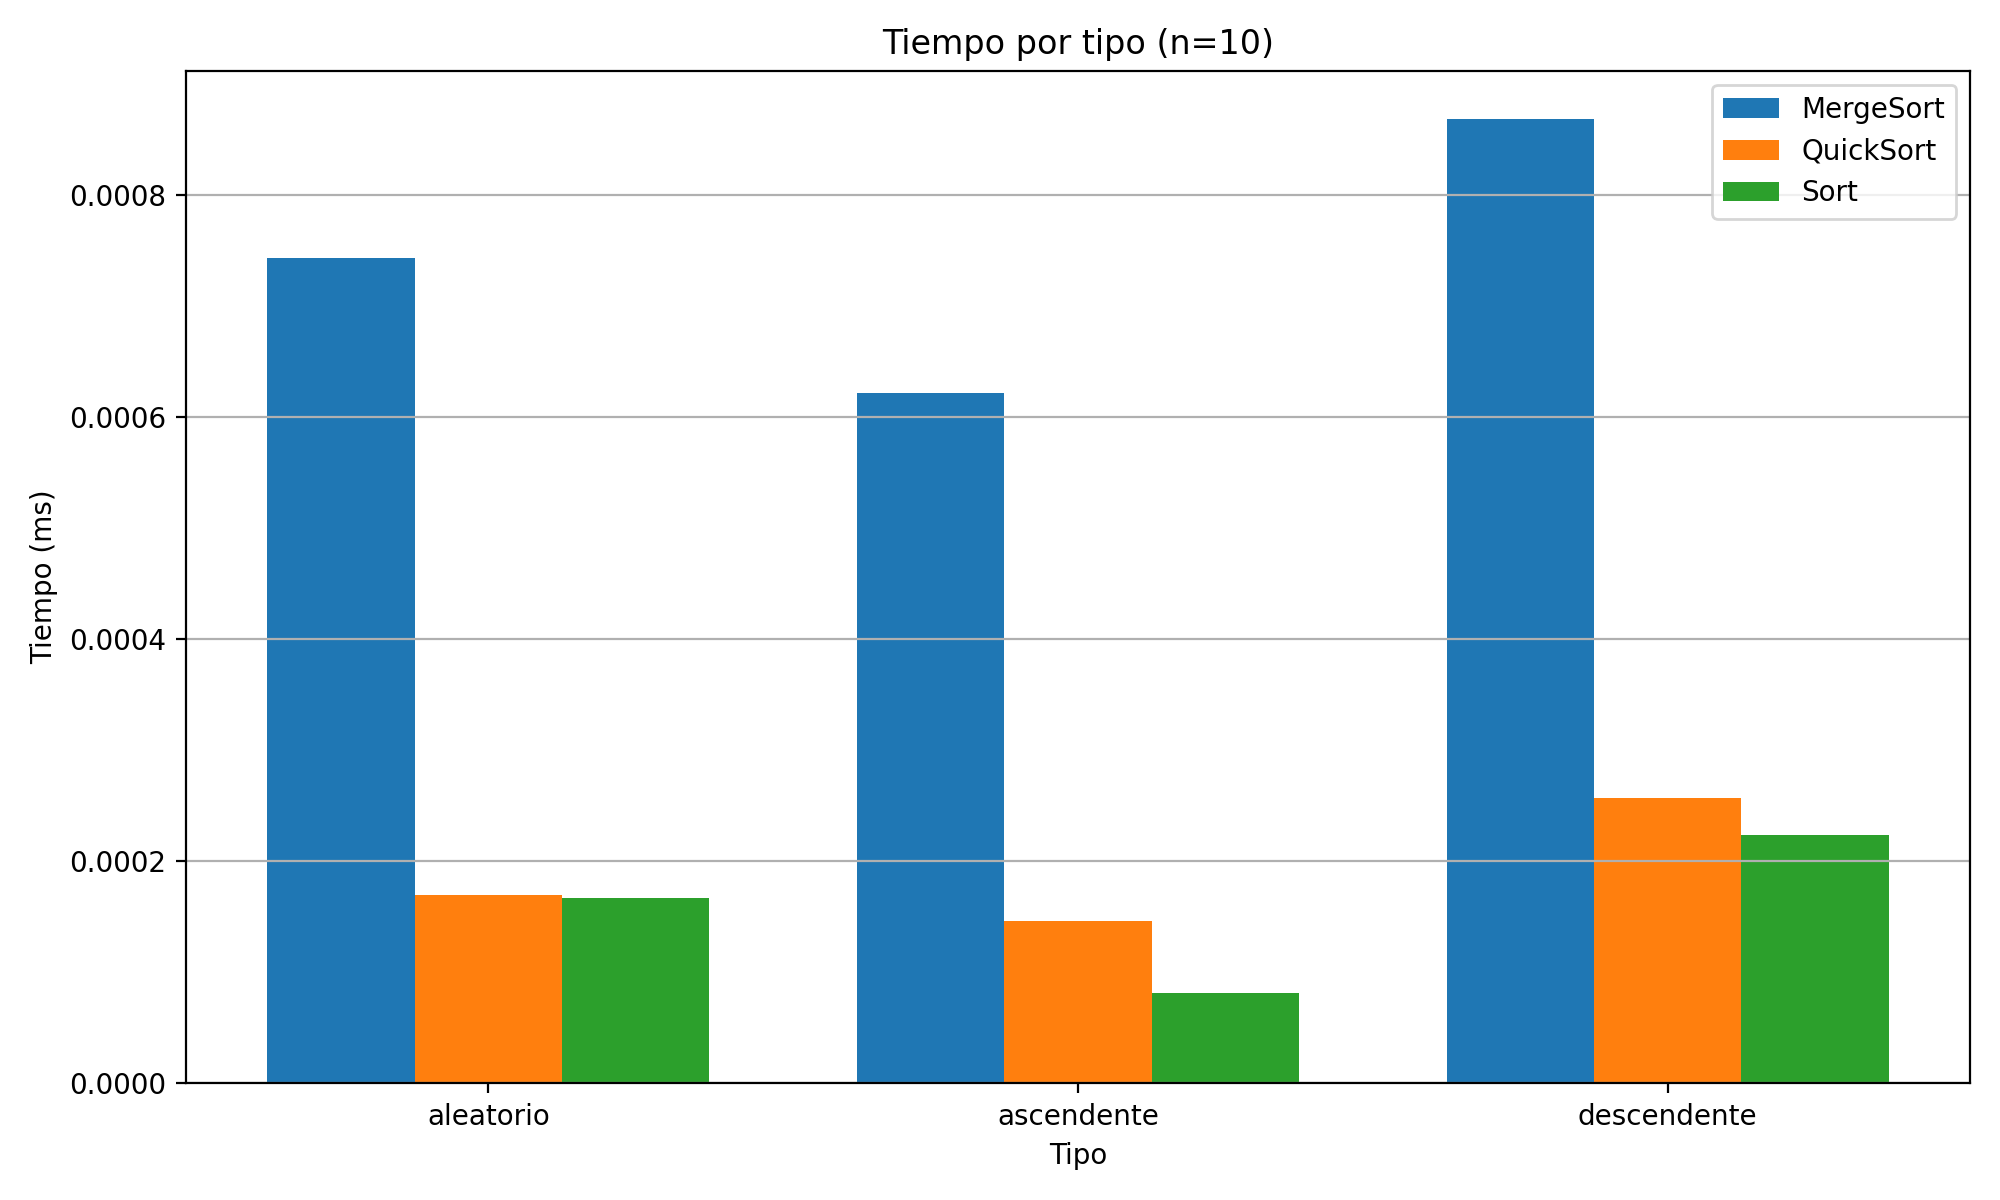
\includegraphics[width=\linewidth]{../code/sorting/data/plots/time_n10.png}
                \caption{Tiempos}
                \label{fig:img2}
            \end{subfigure}

        \end{minipage}
    }
    \caption{Resultados para n=$10^1$}
    \label{fig:comparacion n=$10^1$ sort}
\end{figure}
Para \(n = 10^1\), MergeSort utiliza cerca de \(4n\) bytes de memoria auxiliar, mientras que QuickSort y \texttt{Sort} no presentan uso significativo de heap. 
En tiempo de ejecución, MergeSort resulta ser el más lento en los tres casos, debido al costo de copiar y mezclar subarreglos. 
En cambio, QuickSort y \texttt{Sort} muestran tiempos menores y similares entre sí, con mejor desempeño en el caso ascendente y 
un leve aumento en el descendente, lo que puede explicarse por la forma en que la elección del pivote afecta el balance de las particiones.

\begin{figure}[H]
    \centering
    \resizebox{\textwidth}{!}{
        \begin{minipage}{\textwidth}
            \centering

            \begin{subfigure}{0.48\textwidth}
                \centering
                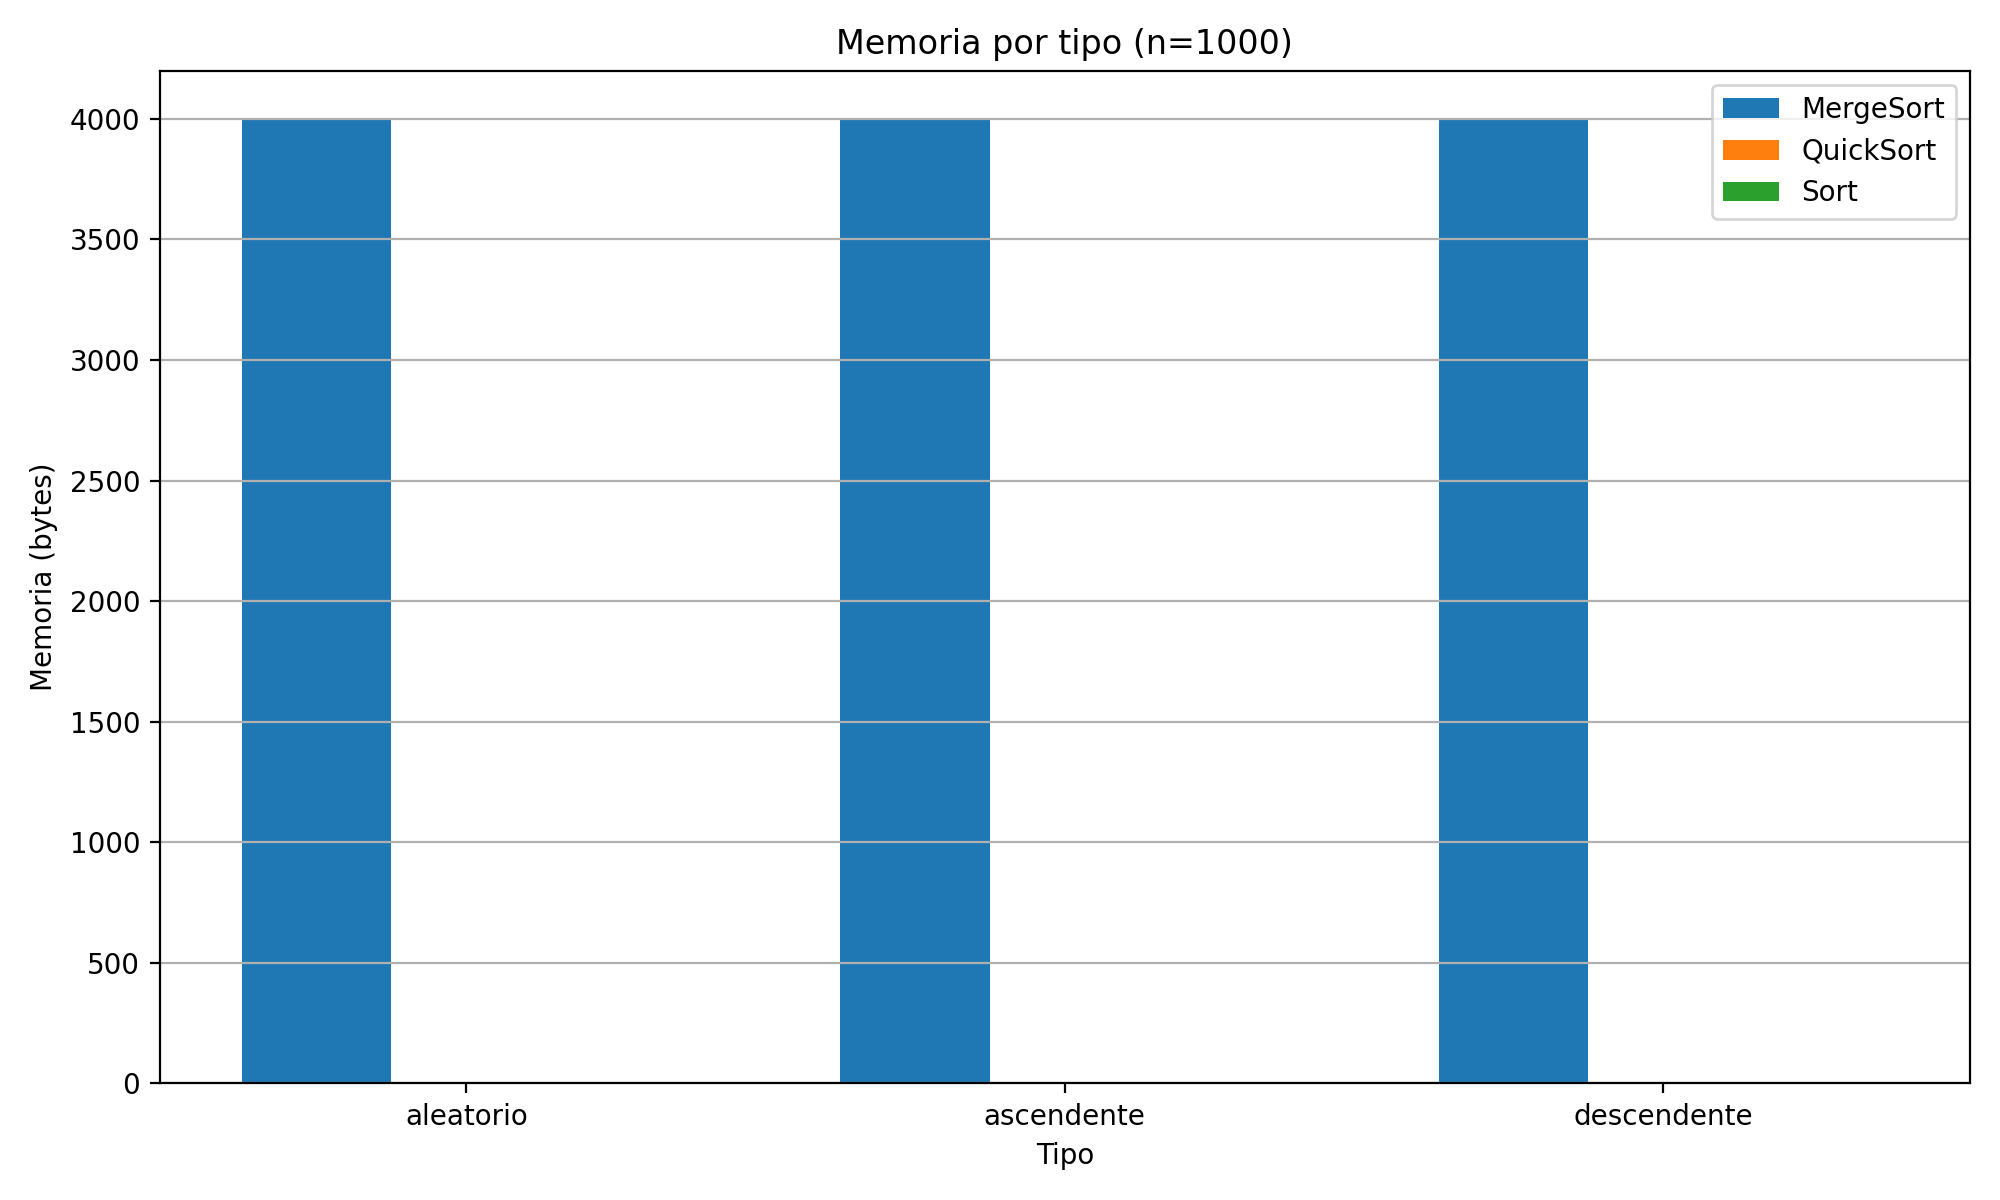
\includegraphics[width=\linewidth]{../code/sorting/data/plots/memory_n1000.png}
                \caption{Memoria}
                \label{fig:img3}
            \end{subfigure}
            \hfill
            \begin{subfigure}{0.48\textwidth}
                \centering
                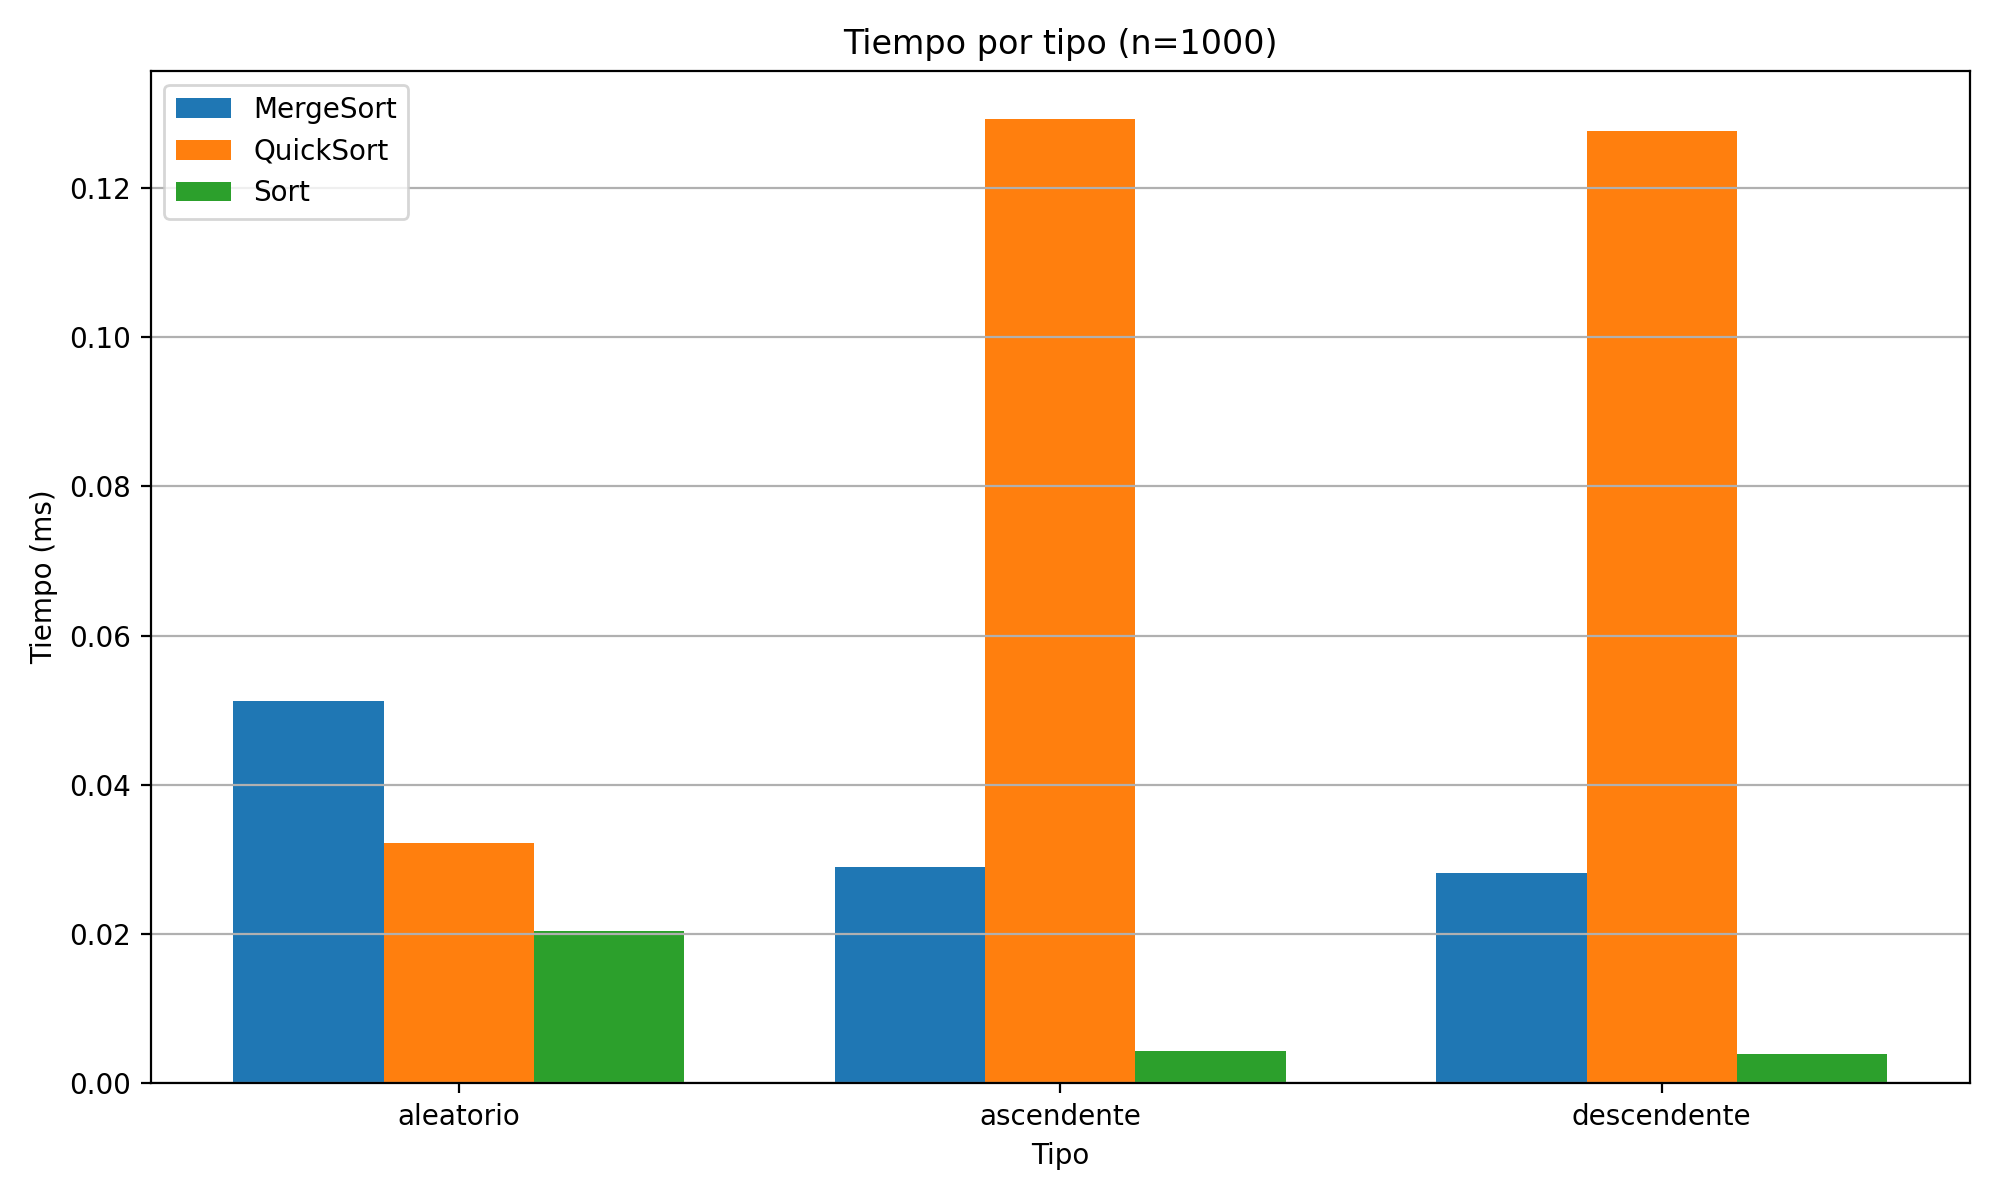
\includegraphics[width=\linewidth]{../code/sorting/data/plots/time_n1000.png}
                \caption{Tiempos}
                \label{fig:img4}
            \end{subfigure}

        \end{minipage}
    }
    \caption{Resultados para n=$10^3$}
    \label{fig:comparacion n=$10^3$ sort}
\end{figure}

Para \(n = 10^3\), MergeSort utiliza aproximadamente \(4n\) bytes de memoria auxiliar, mientras que QuickSort y 
\texttt{Sort} no presentan uso significativo de heap. En tiempo de ejecución, MergeSort mantiene un comportamiento estable en todos los casos.
QuickSort, en cambio, presenta un buen desempeño en el caso promedio, pero se degrada fuertemente en entradas ascendentes y descendentes 
debido a la mala elección de pivote. Finalmente, \texttt{Sort} obtiene los mejores tiempos en todos los casos, gracias a su 
implementación híbrida que evita el peor caso.

\begin{figure}[H]
    \centering
    \resizebox{\textwidth}{!}{
        \begin{minipage}{\textwidth}
            \centering

            \begin{subfigure}{0.48\textwidth}
                \centering
                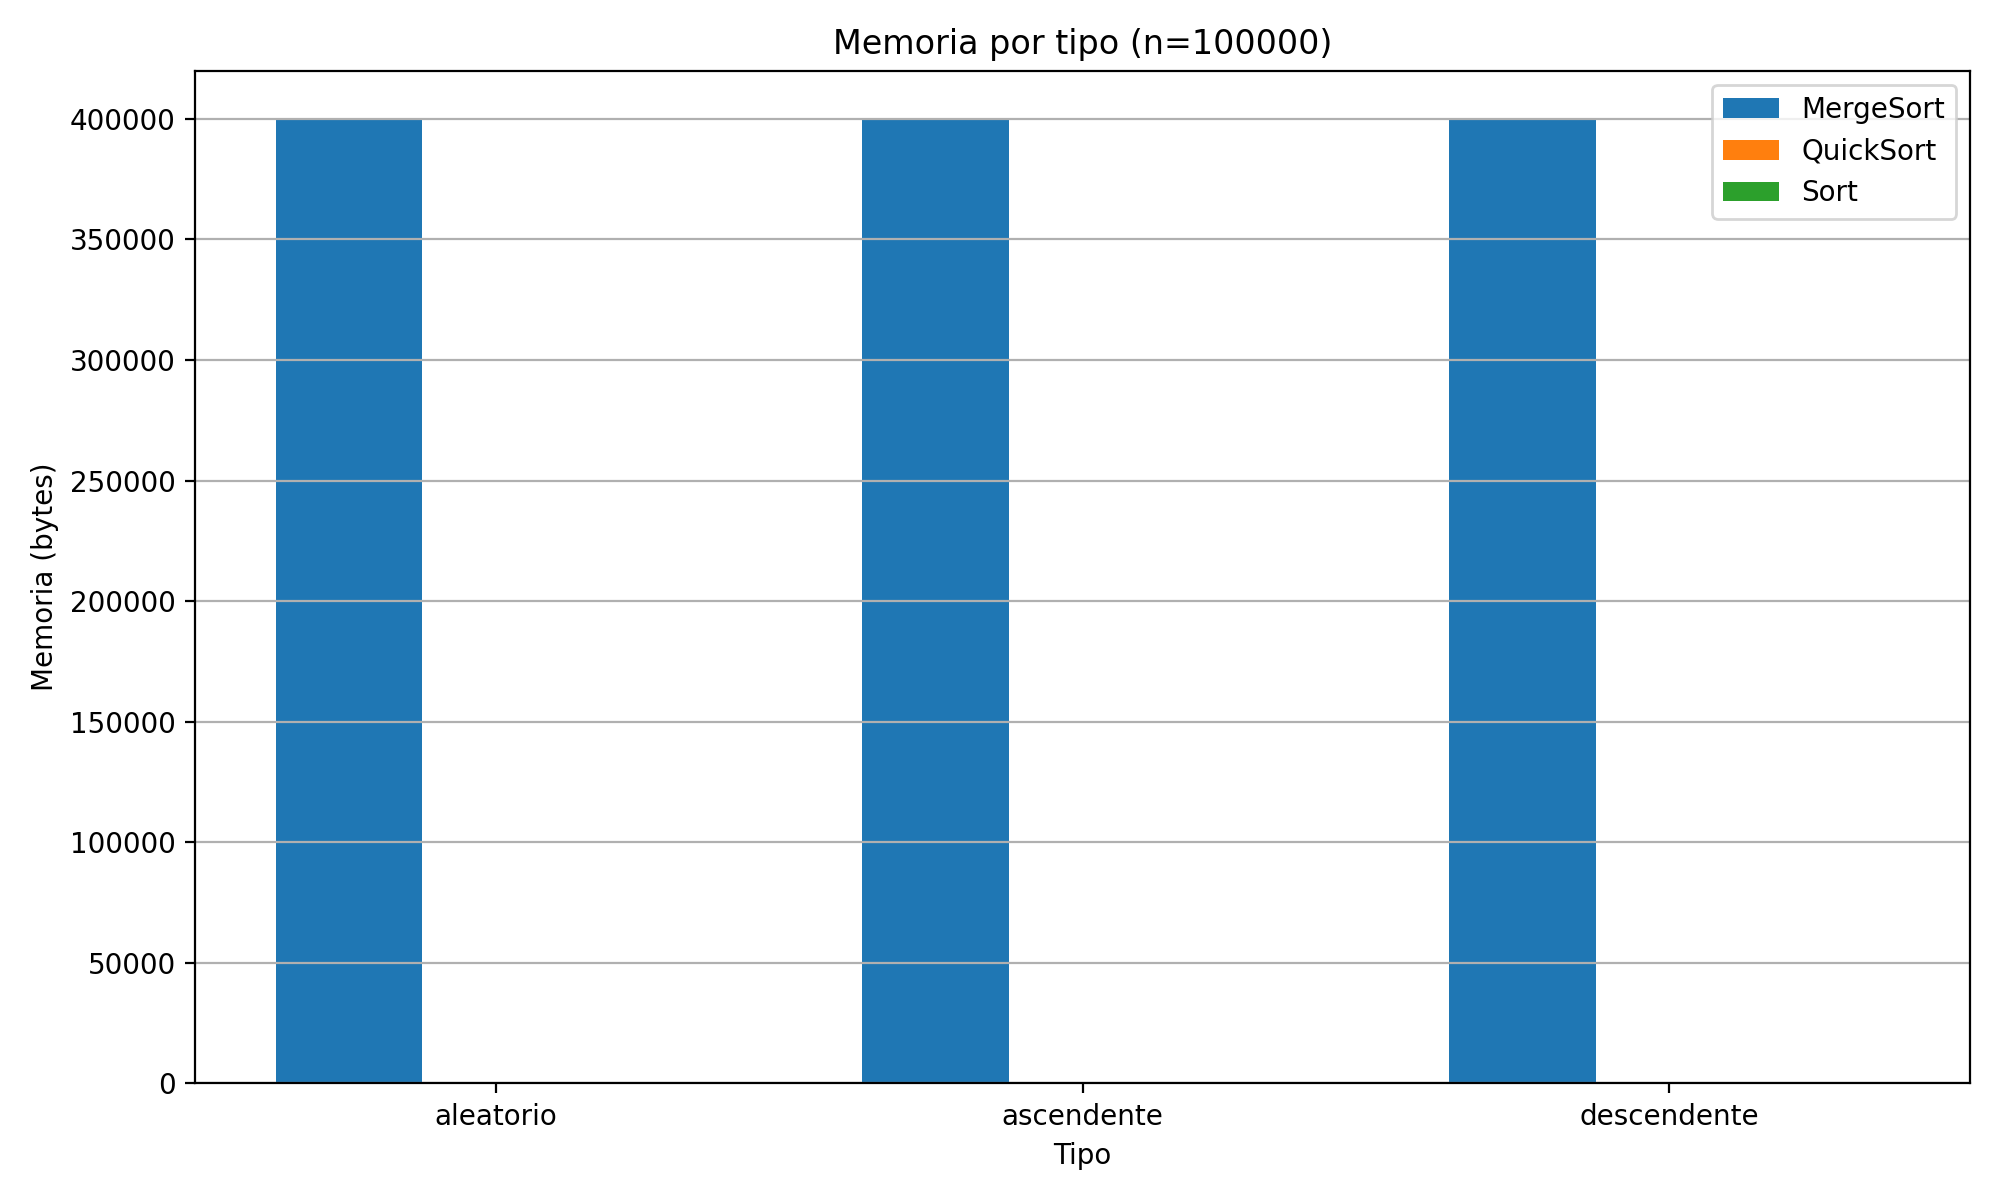
\includegraphics[width=\linewidth]{../code/sorting/data/plots/memory_n100000.png}
                \caption{Memoria}
                \label{fig:img5}
            \end{subfigure}
            \hfill
            \begin{subfigure}{0.48\textwidth}
                \centering
                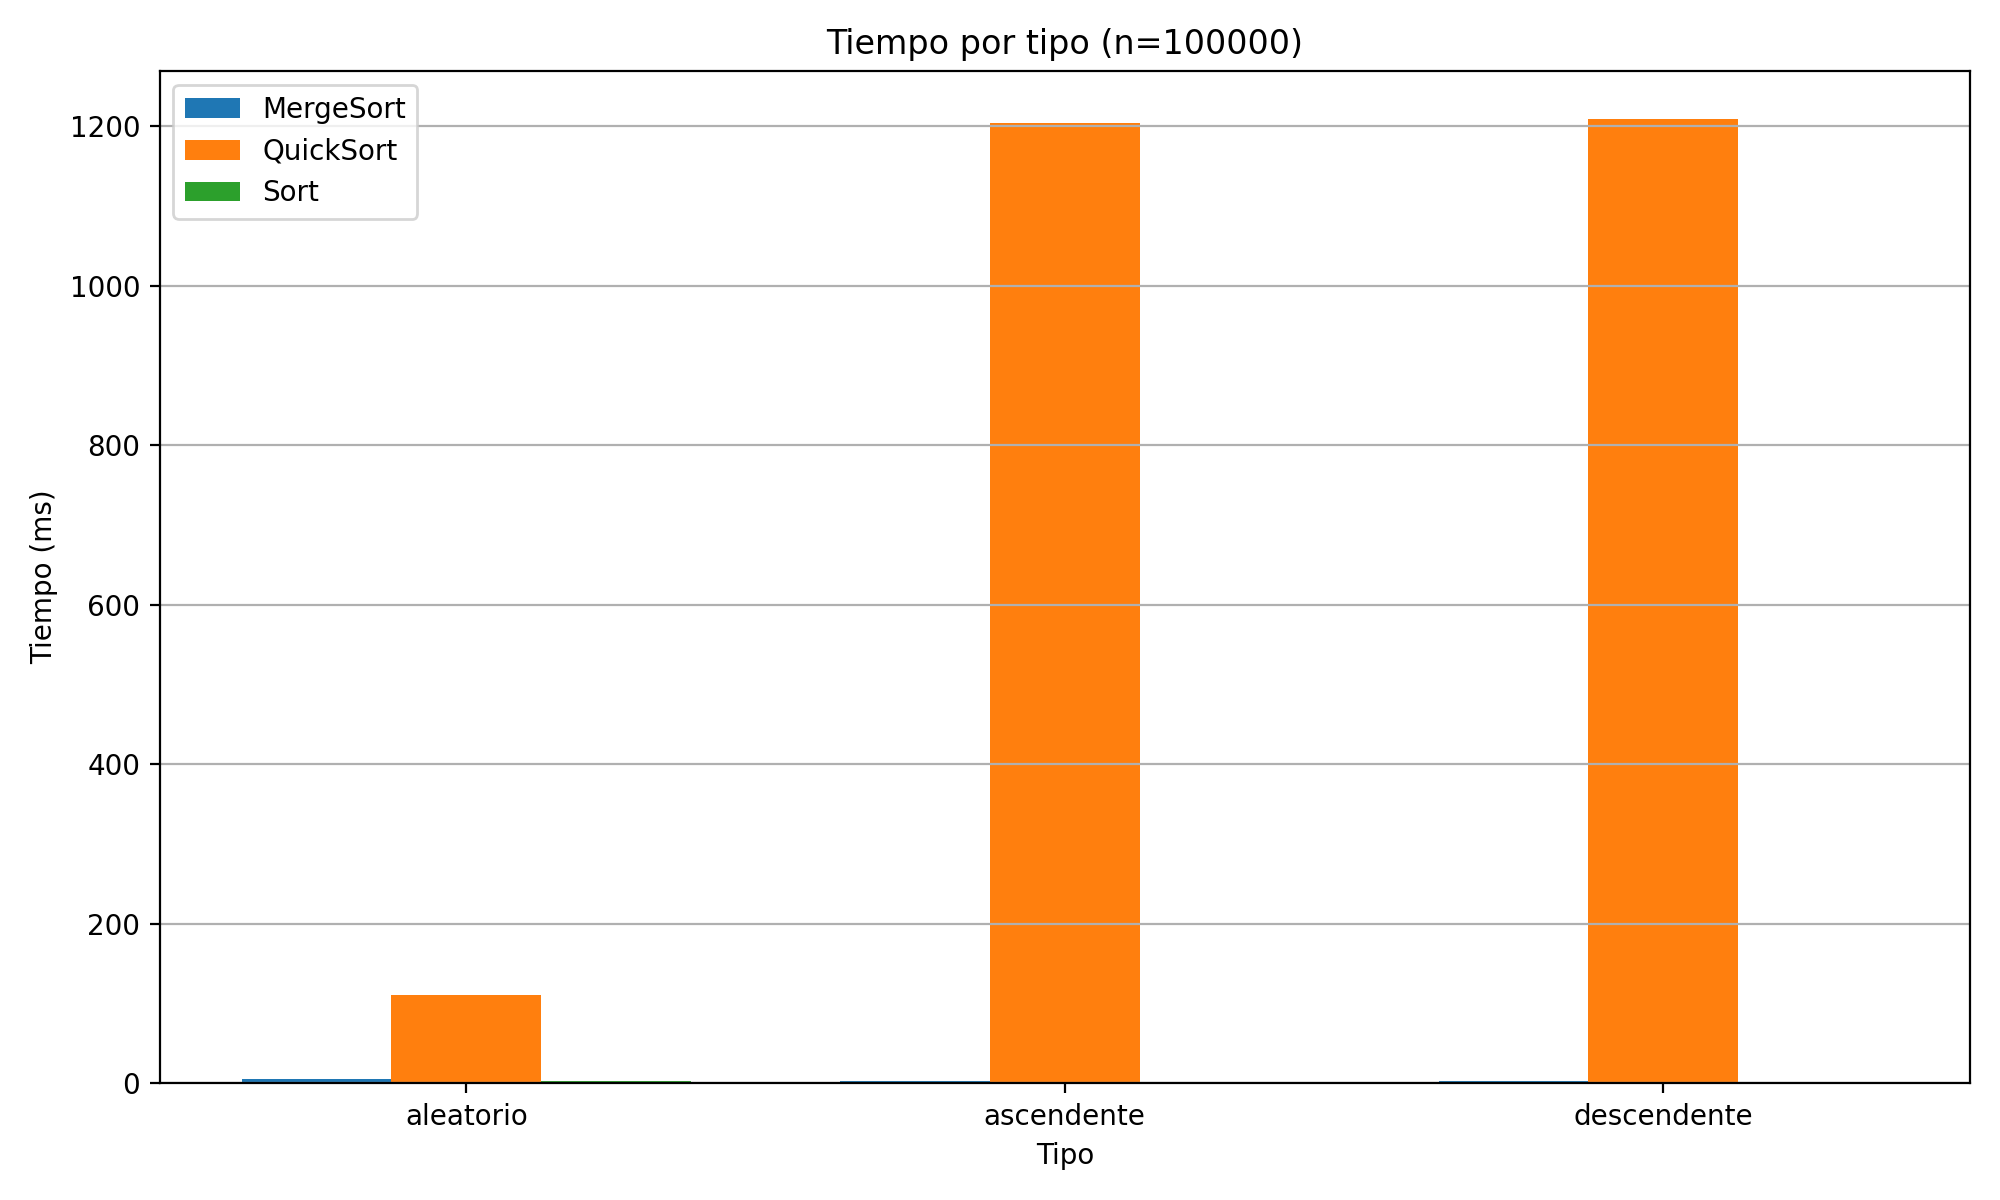
\includegraphics[width=\linewidth]{../code/sorting/data/plots/time_n100000.png}
                \caption{Tiempos}
                \label{fig:img6}
            \end{subfigure}

        \end{minipage}
    }
    \caption{Resultados para n=$10^5$}
    \label{fig:comparacion n=$10^5$ sort} 
\end{figure}
Para \(n = 10^5\), el comportamiento de la memoria se mantiene igual que en los casos anteriores. 
Sin embargo, destaca el bajo rendimiento de QuickSort en los casos ascendente y descendente, cuyos tiempos crecen de tal forma que 
dejan fuera de escala los de MergeSort y \texttt{sort} en la gráfica.
\\ 
En un análisis general, se observa que QuickSort presenta un mal rendimiento cuando el arreglo está ordenado de forma ascendente o 
descendente, ya que en estos casos su complejidad se degrada a \(O(n^2)\), lo que se acentúa al aumentar \(n\). 
Por otro lado, \texttt{sort} mantiene un buen desempeño en todos los casos gracias a su implementación híbrida, 
que evita el peor caso de QuickSort. Finalmente, MergeSort presenta tiempos estables independientes del tipo de entrada, aunque su 
principal desventaja es el uso de memoria adicional proporcional al tamaño del arreglo.
\\ 
A continuación, se presenta el análisis de los algoritmos de multiplicación de matrices.
\begin{figure}[H]
    \centering
    \resizebox{\textwidth}{!}{
        \begin{minipage}{\textwidth}
            \centering

            \begin{subfigure}{0.48\textwidth}
                \centering
                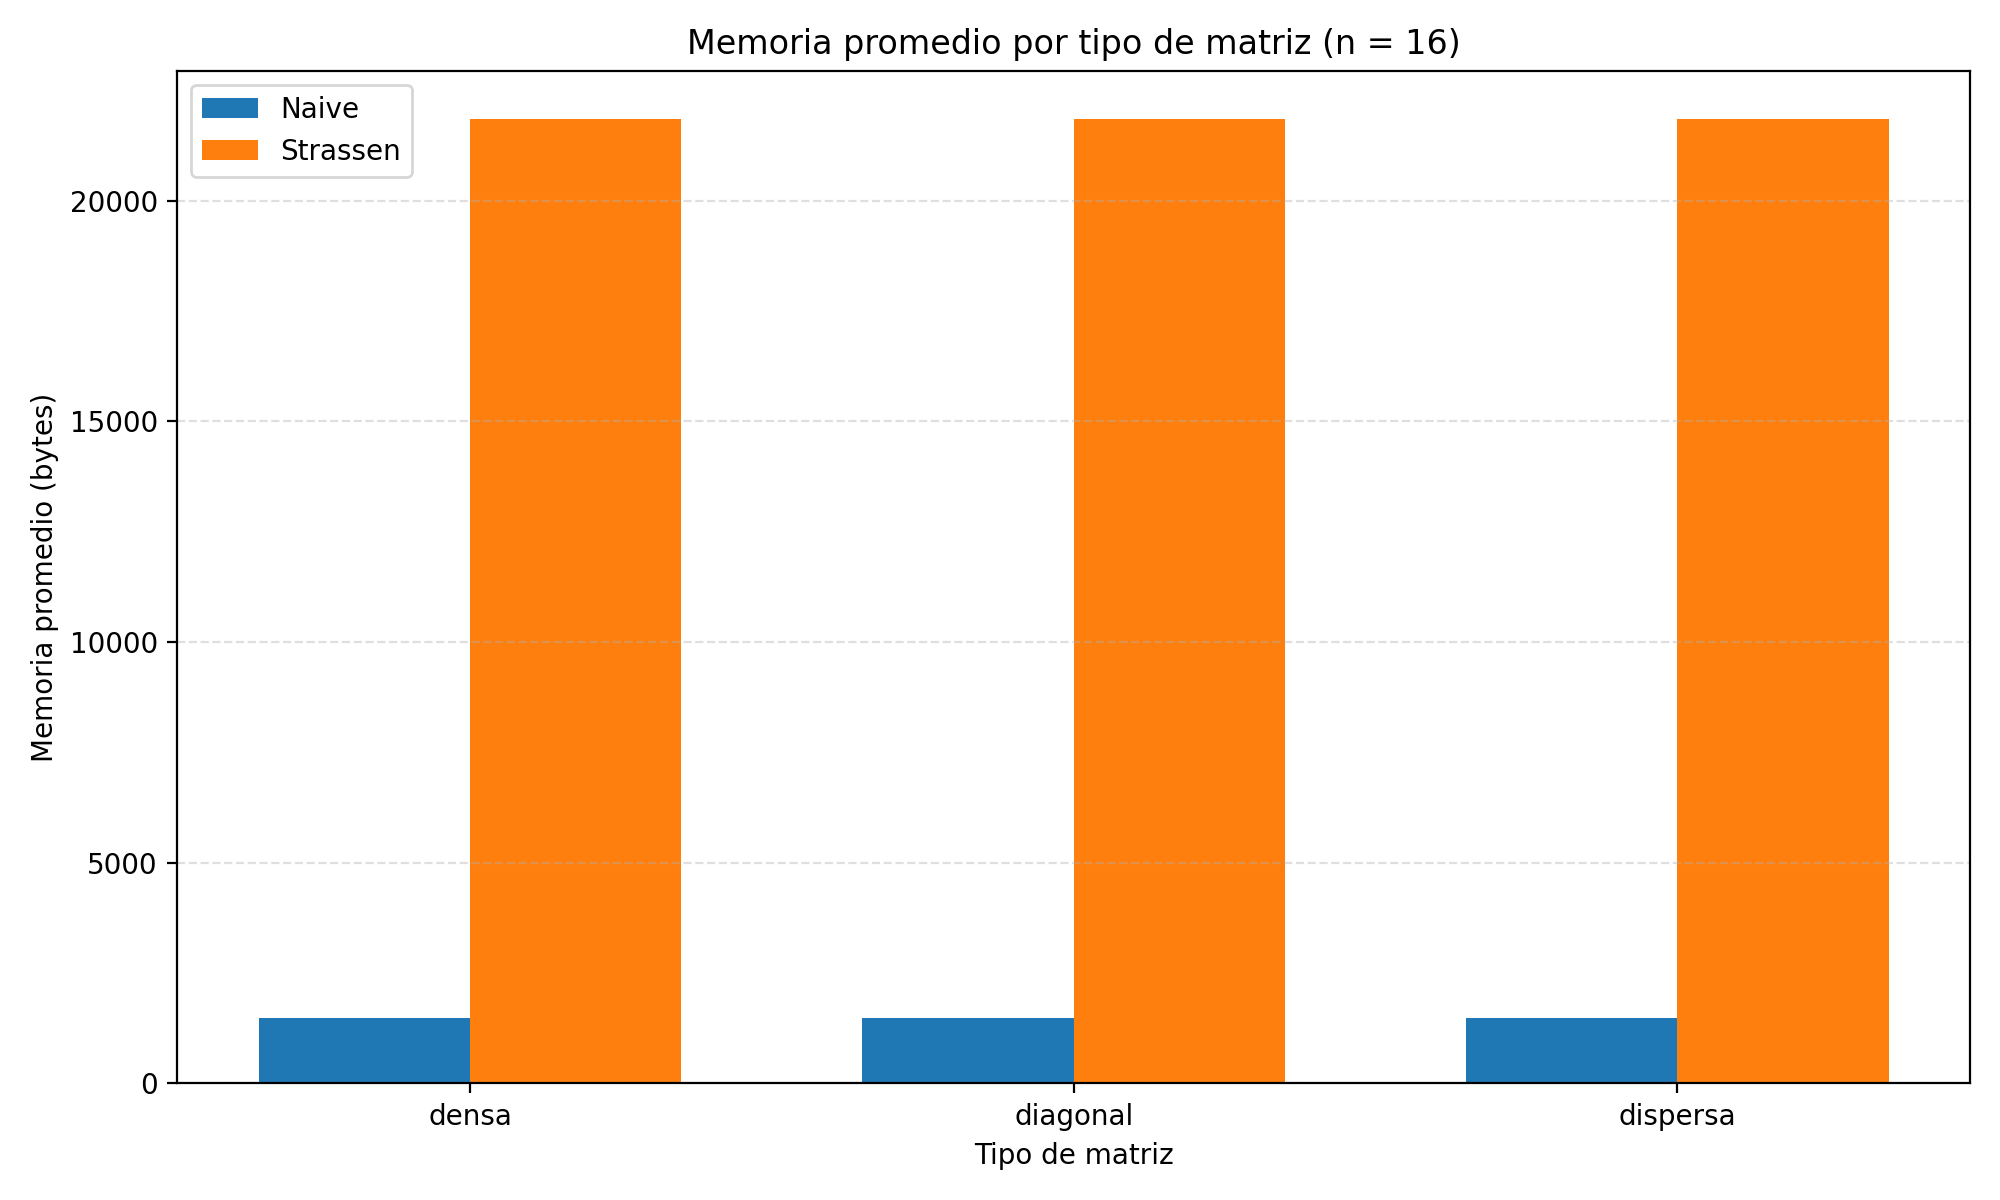
\includegraphics[width=\linewidth]{../code/matrix_multiplication/data/plots/matrix_barras_memoria_n16.png}
                \caption{Memoria}
                \label{fig:img7}
            \end{subfigure}
            \hfill
            \begin{subfigure}{0.48\textwidth}
                \centering
                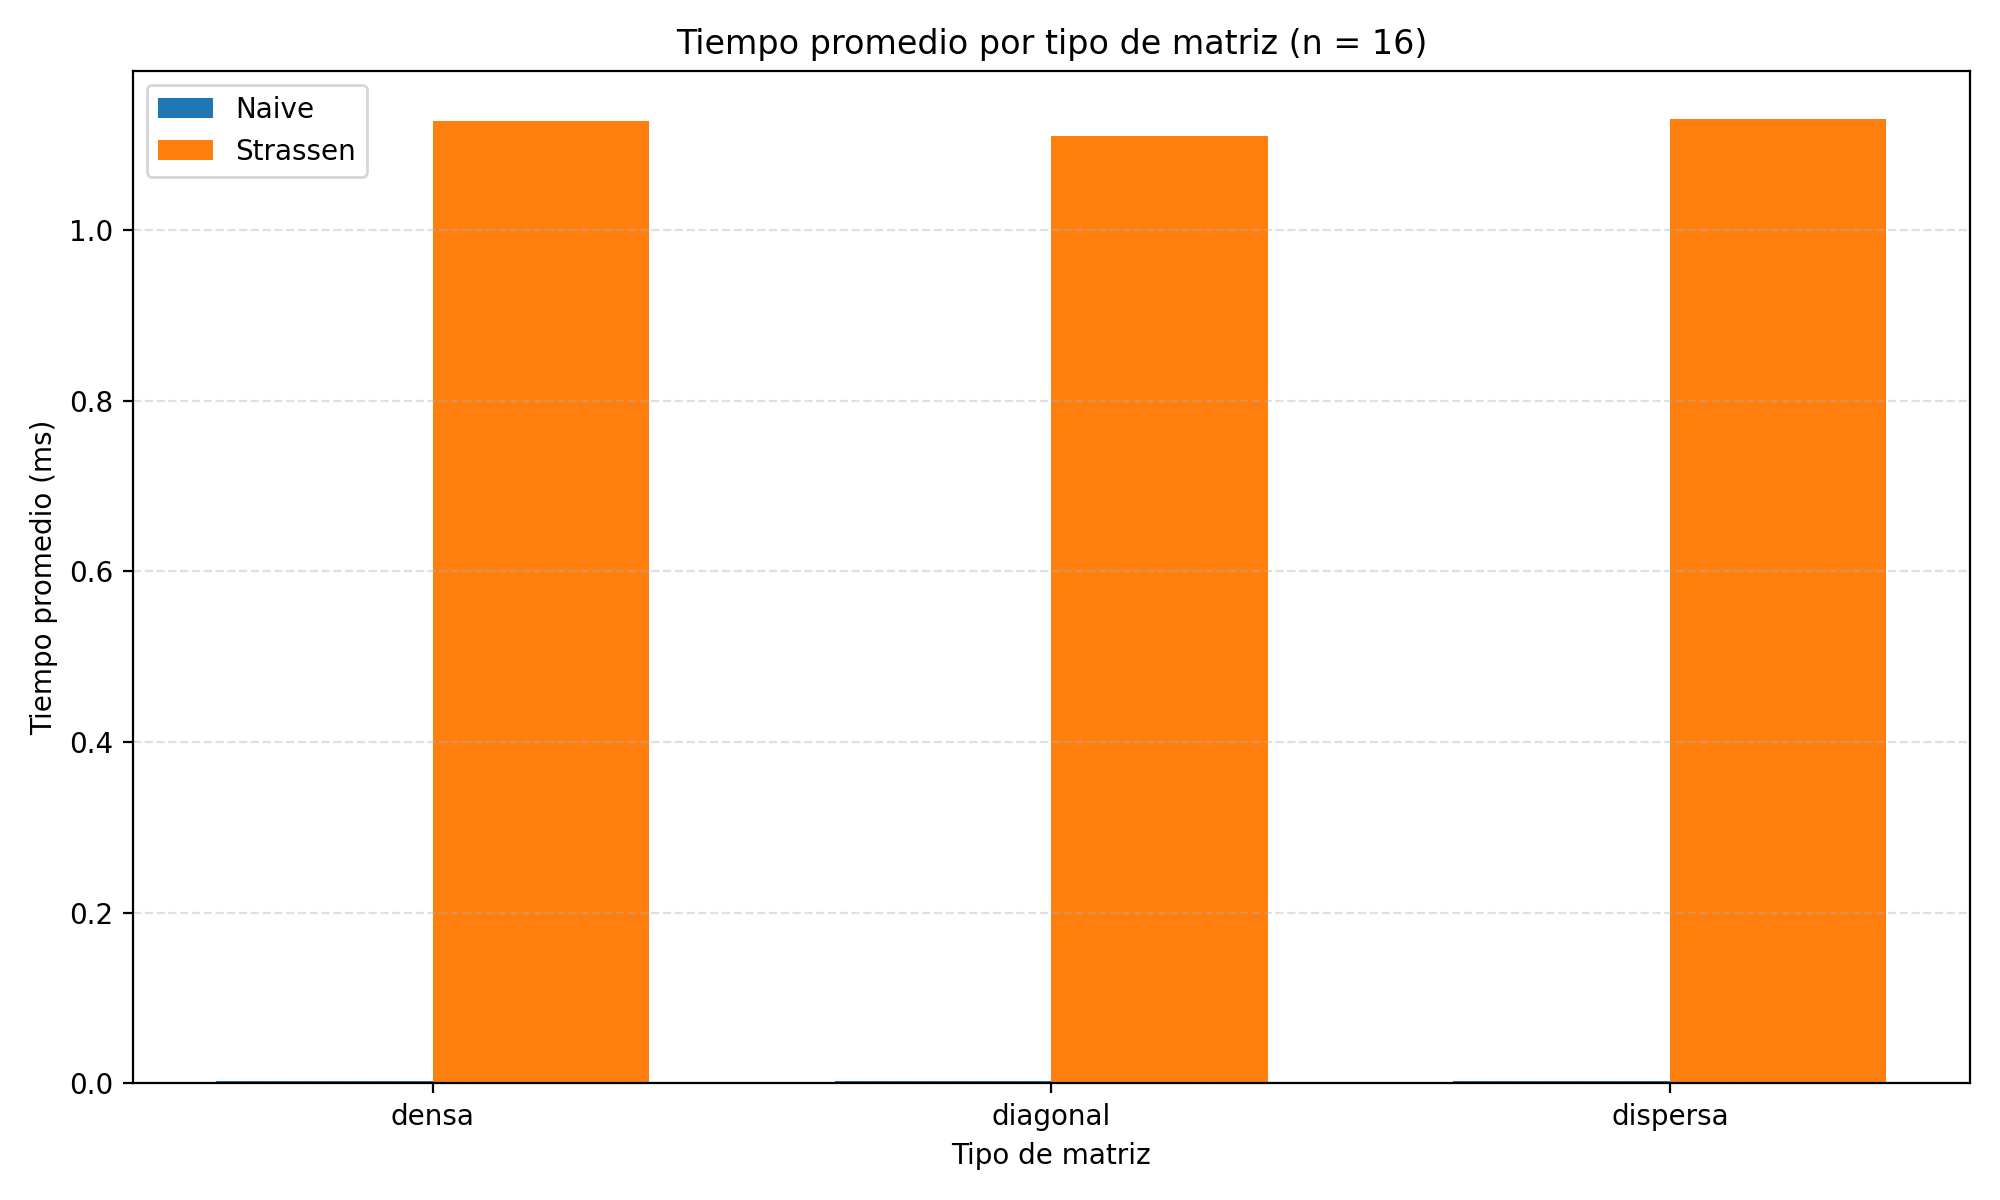
\includegraphics[width=\linewidth]{../code/matrix_multiplication/data/plots/matrix_barras_tiempo_n16.png}
                \caption{Tiempos}
                \label{fig:img8}
            \end{subfigure}

        \end{minipage}
    }
    \caption{Resultados para matrices 16x16}
    \label{fig:comparacion 16x16 matrix}
\end{figure}


\begin{figure}[H]
    \centering
    \resizebox{\textwidth}{!}{
        \begin{minipage}{\textwidth}
            \centering

            \begin{subfigure}{0.48\textwidth}
                \centering
                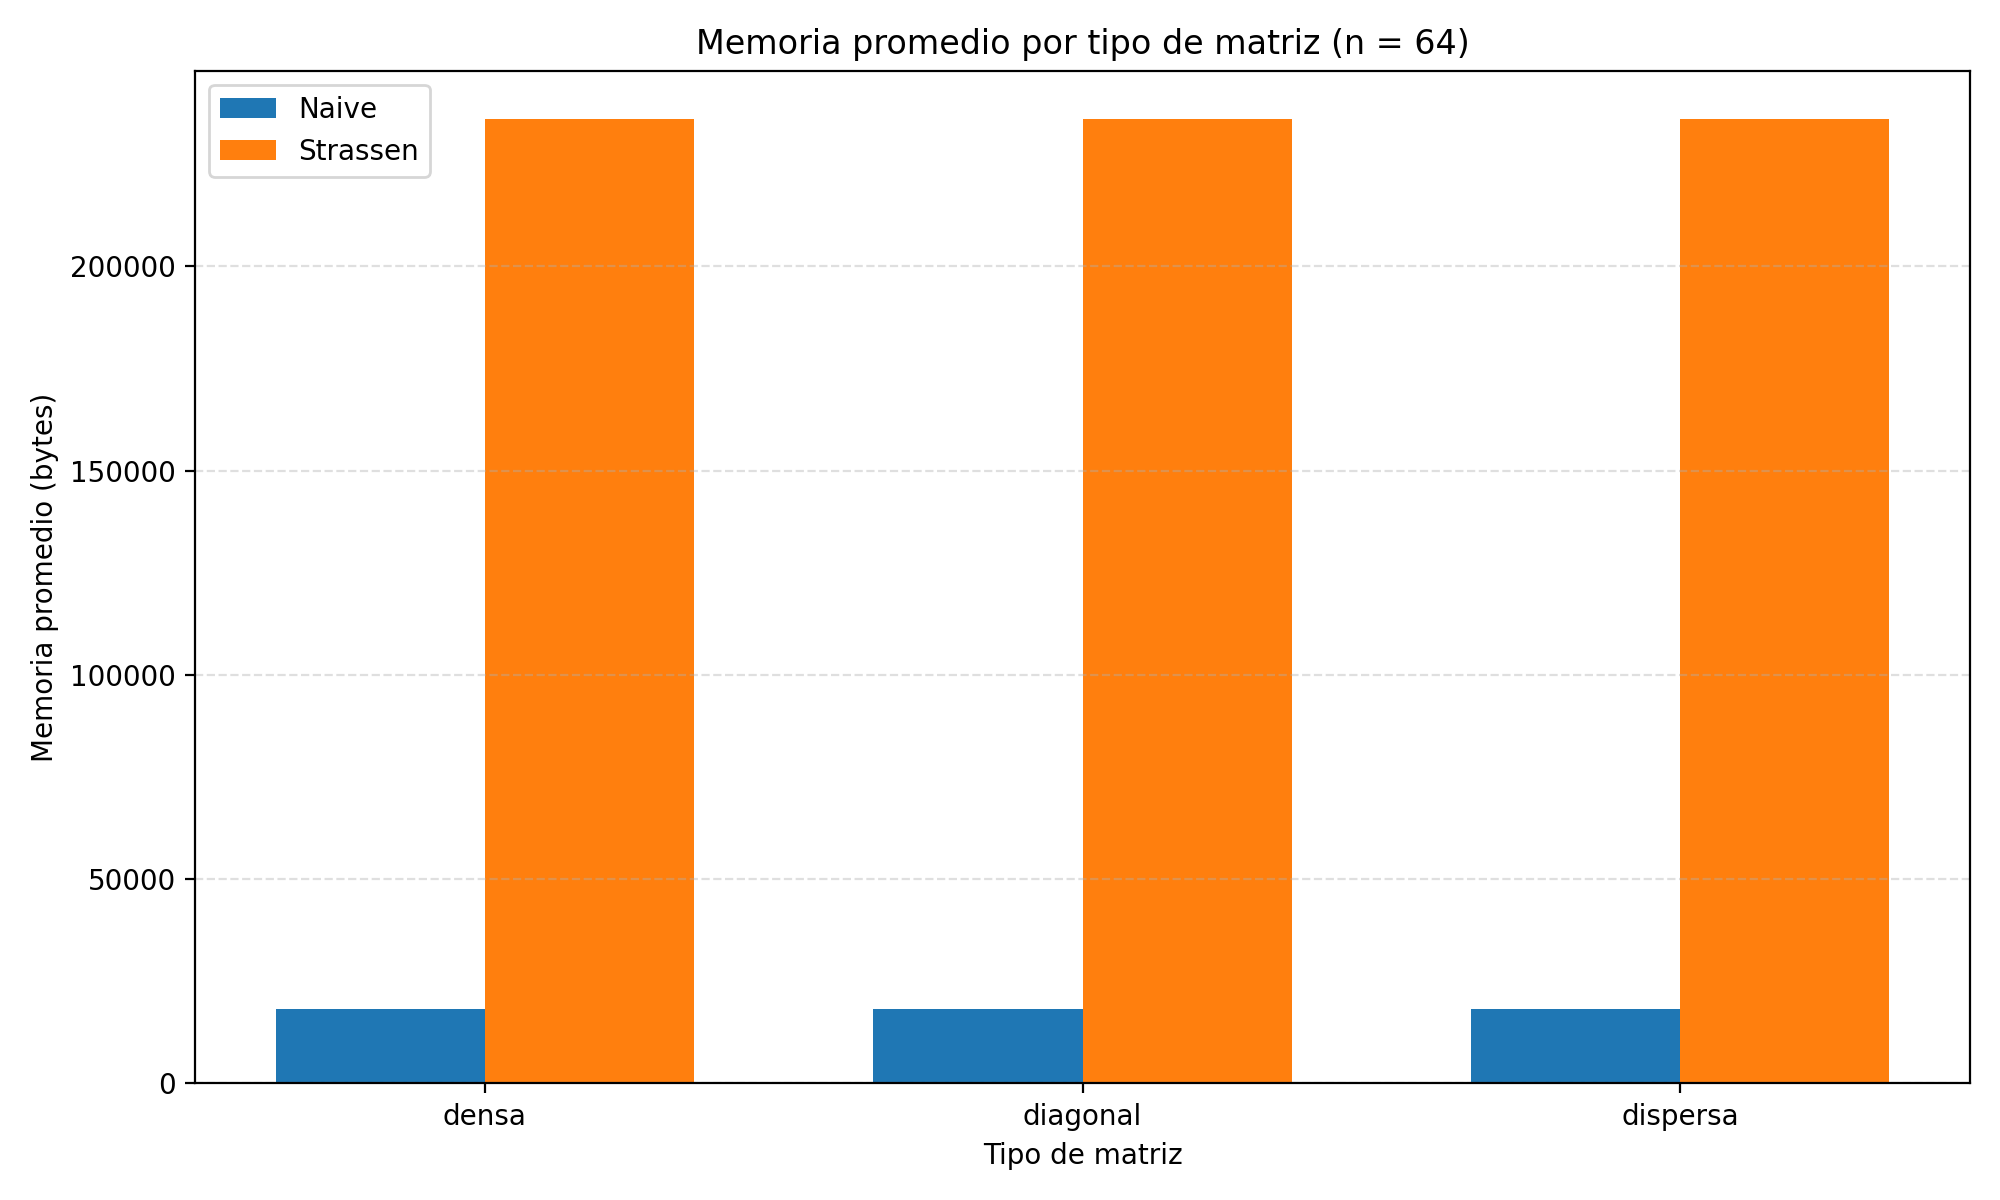
\includegraphics[width=\linewidth]{../code/matrix_multiplication/data/plots/matrix_barras_memoria_n64.png}
                \caption{Memoria}
                \label{fig:img9}
            \end{subfigure}
            \hfill
            \begin{subfigure}{0.48\textwidth}
                \centering
                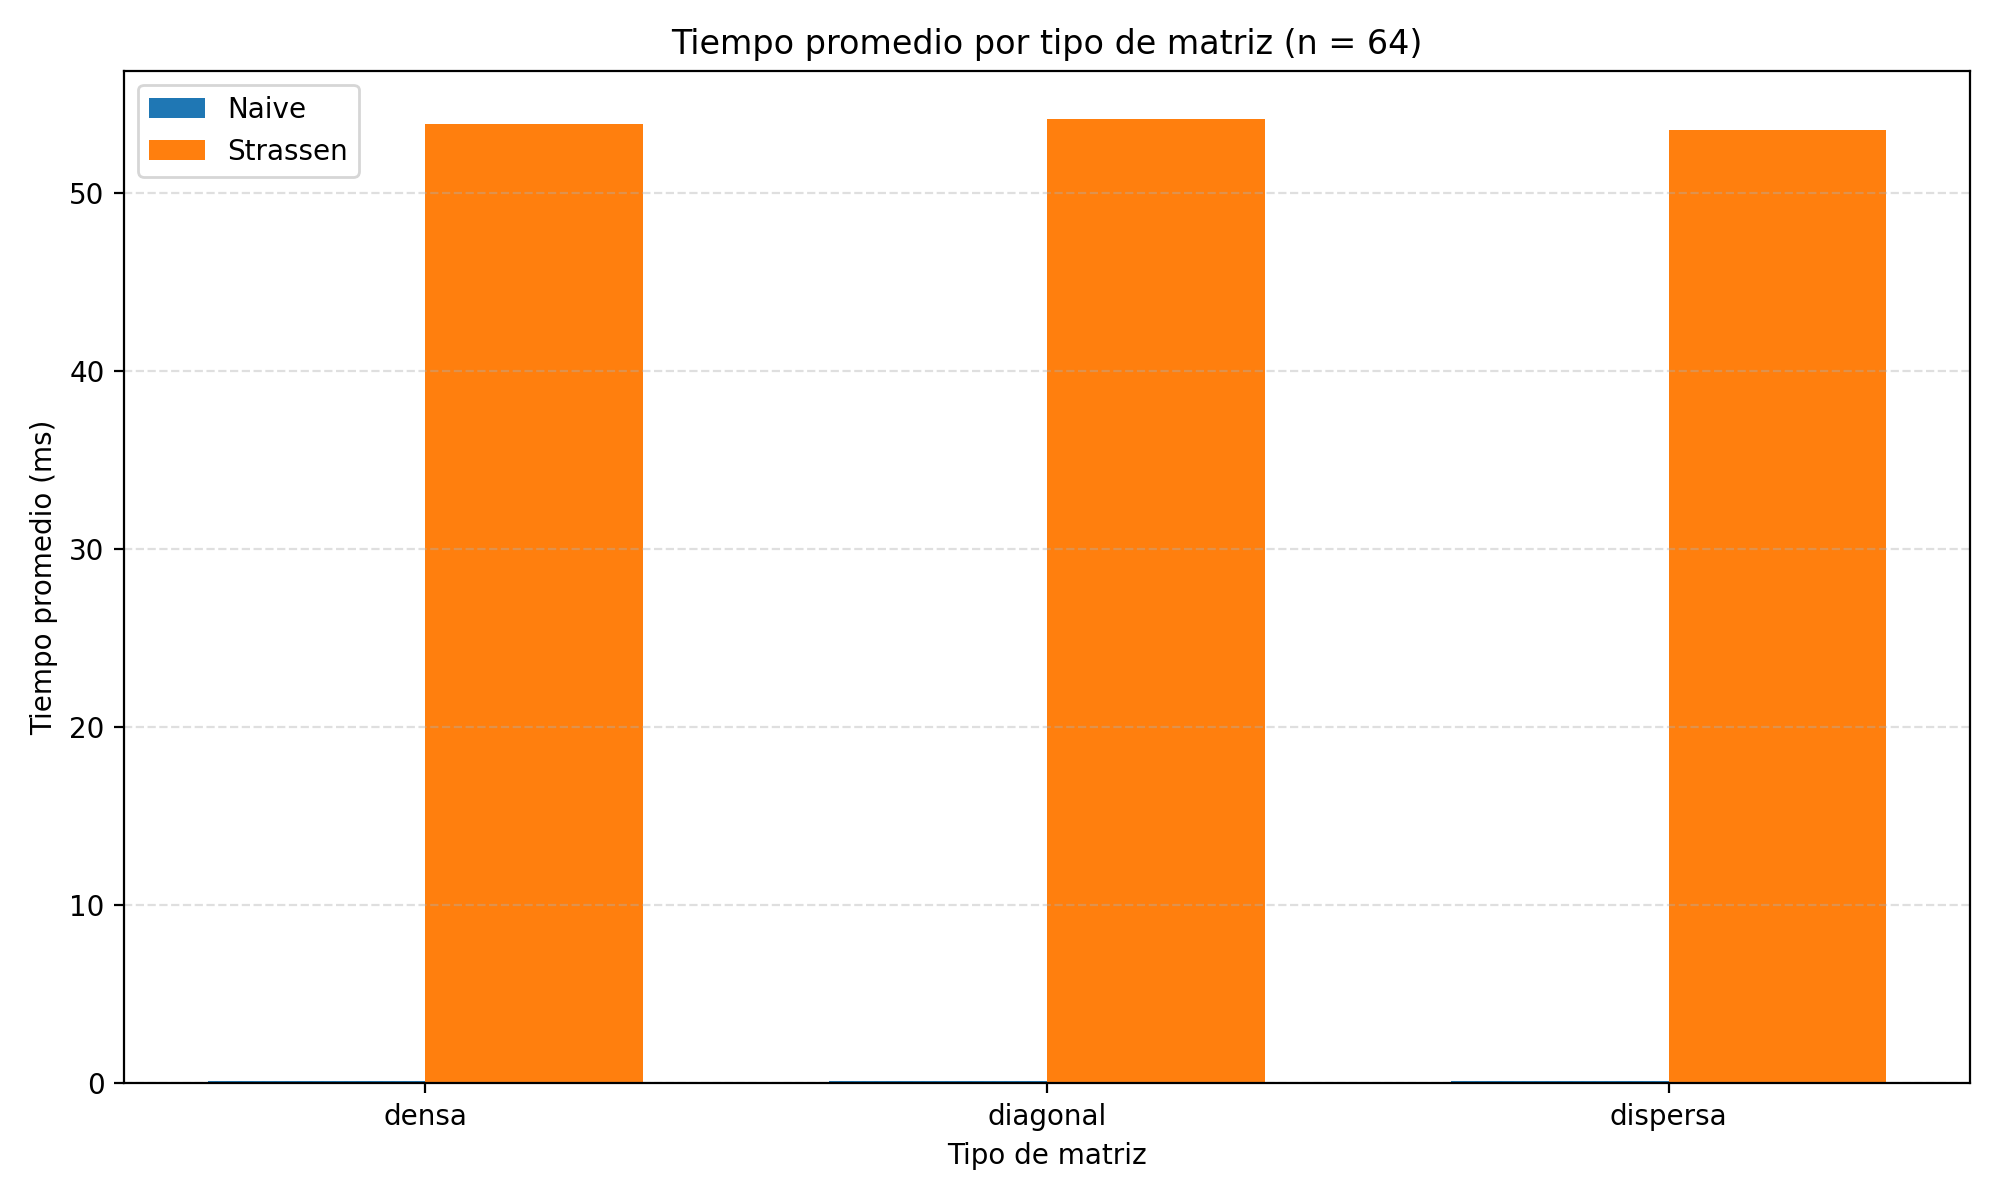
\includegraphics[width=\linewidth]{../code/matrix_multiplication/data/plots/matrix_barras_tiempo_n64.png}
                \caption{Tiempos}
                \label{fig:img10}
            \end{subfigure}

        \end{minipage}
    }
    \caption{Resultados para matrices 64x64}
    \label{fig:comparacion 64x64 matrix}
\end{figure}


\begin{figure}[H]
    \centering
    \resizebox{\textwidth}{!}{
        \begin{minipage}{\textwidth}
            \centering

            \begin{subfigure}{0.48\textwidth}
                \centering
                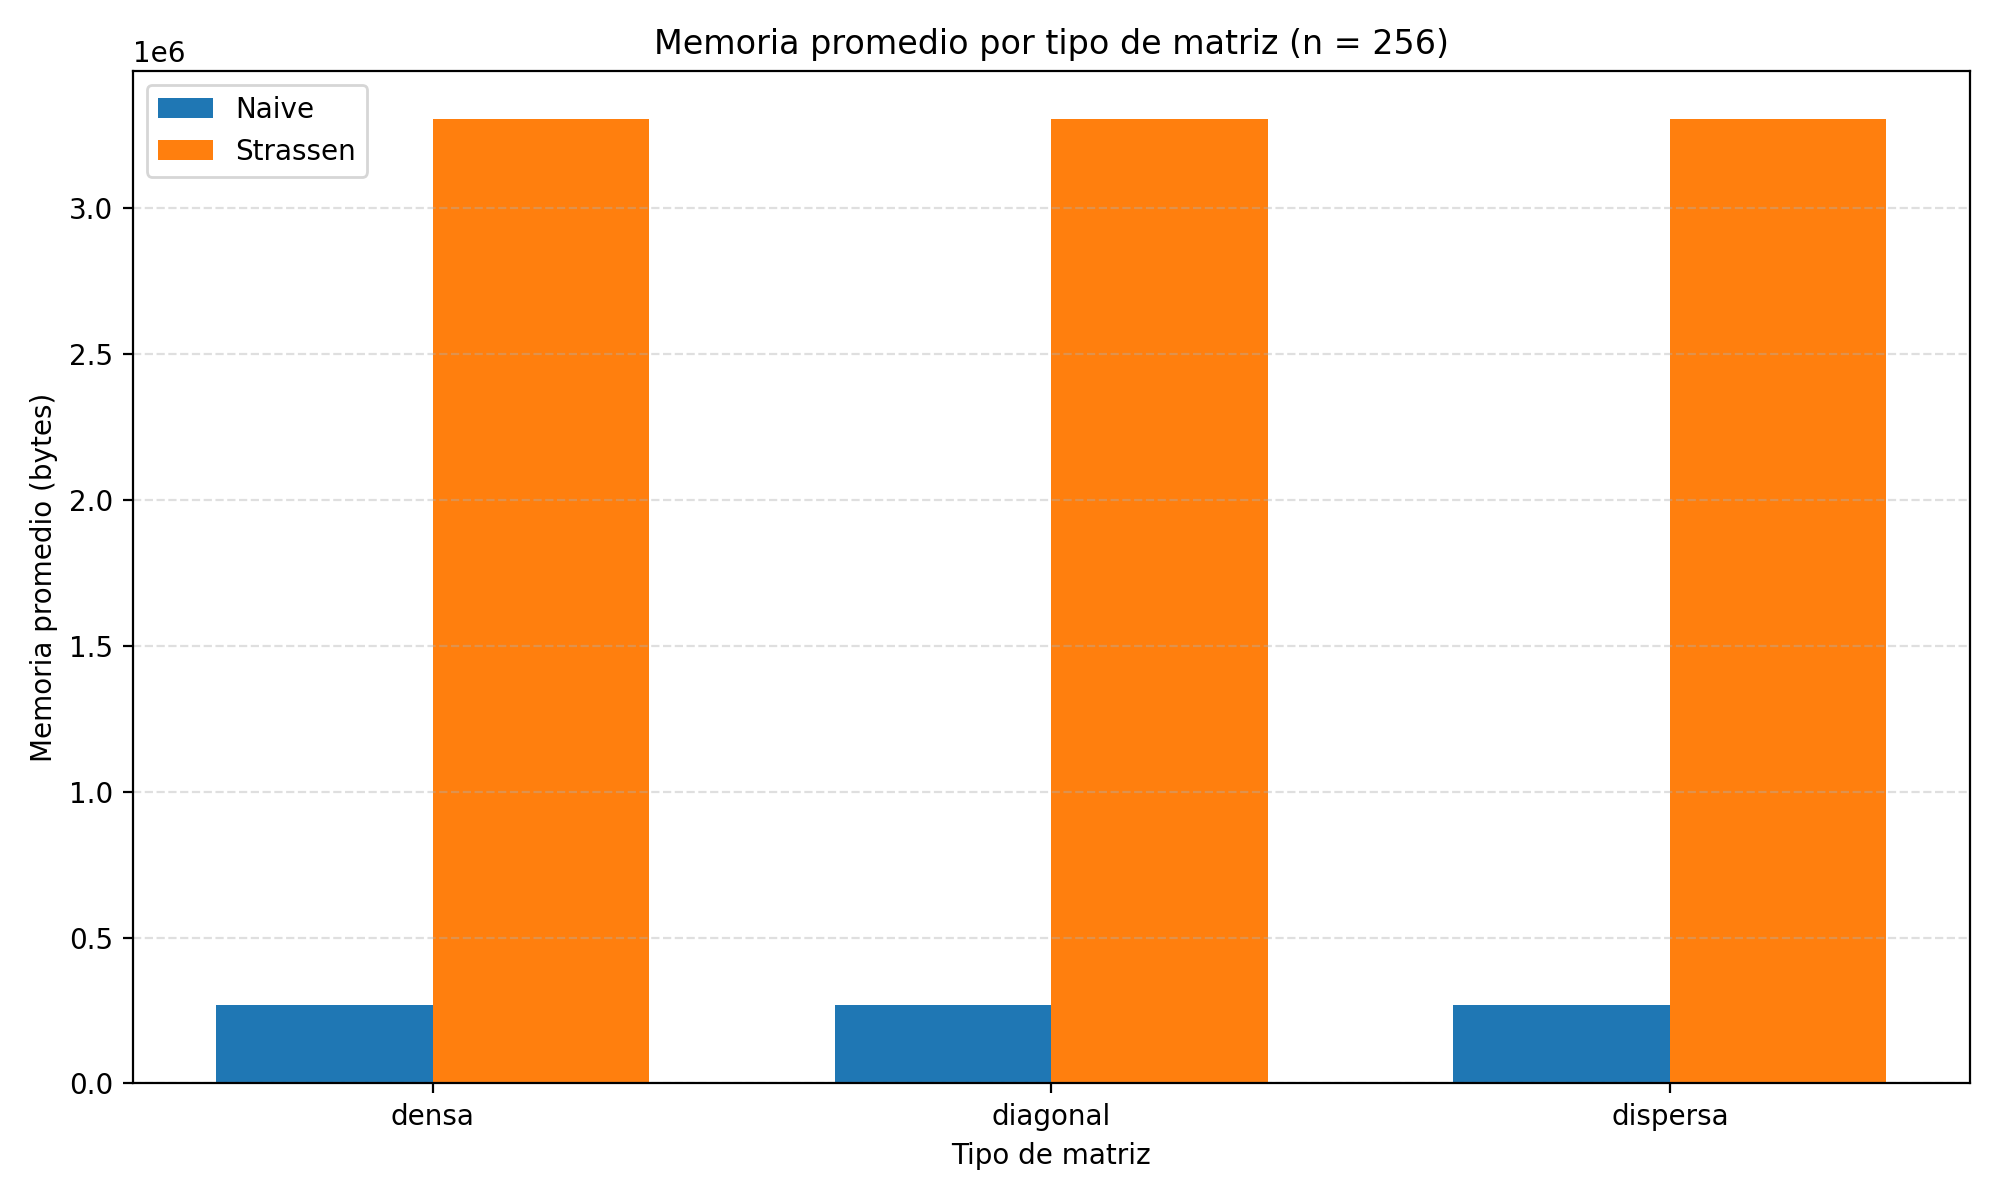
\includegraphics[width=\linewidth]{../code/matrix_multiplication/data/plots/matrix_barras_memoria_n256.png}
                \caption{Memoria}
                \label{fig:img11}
            \end{subfigure}
            \hfill
            \begin{subfigure}{0.48\textwidth}
                \centering
                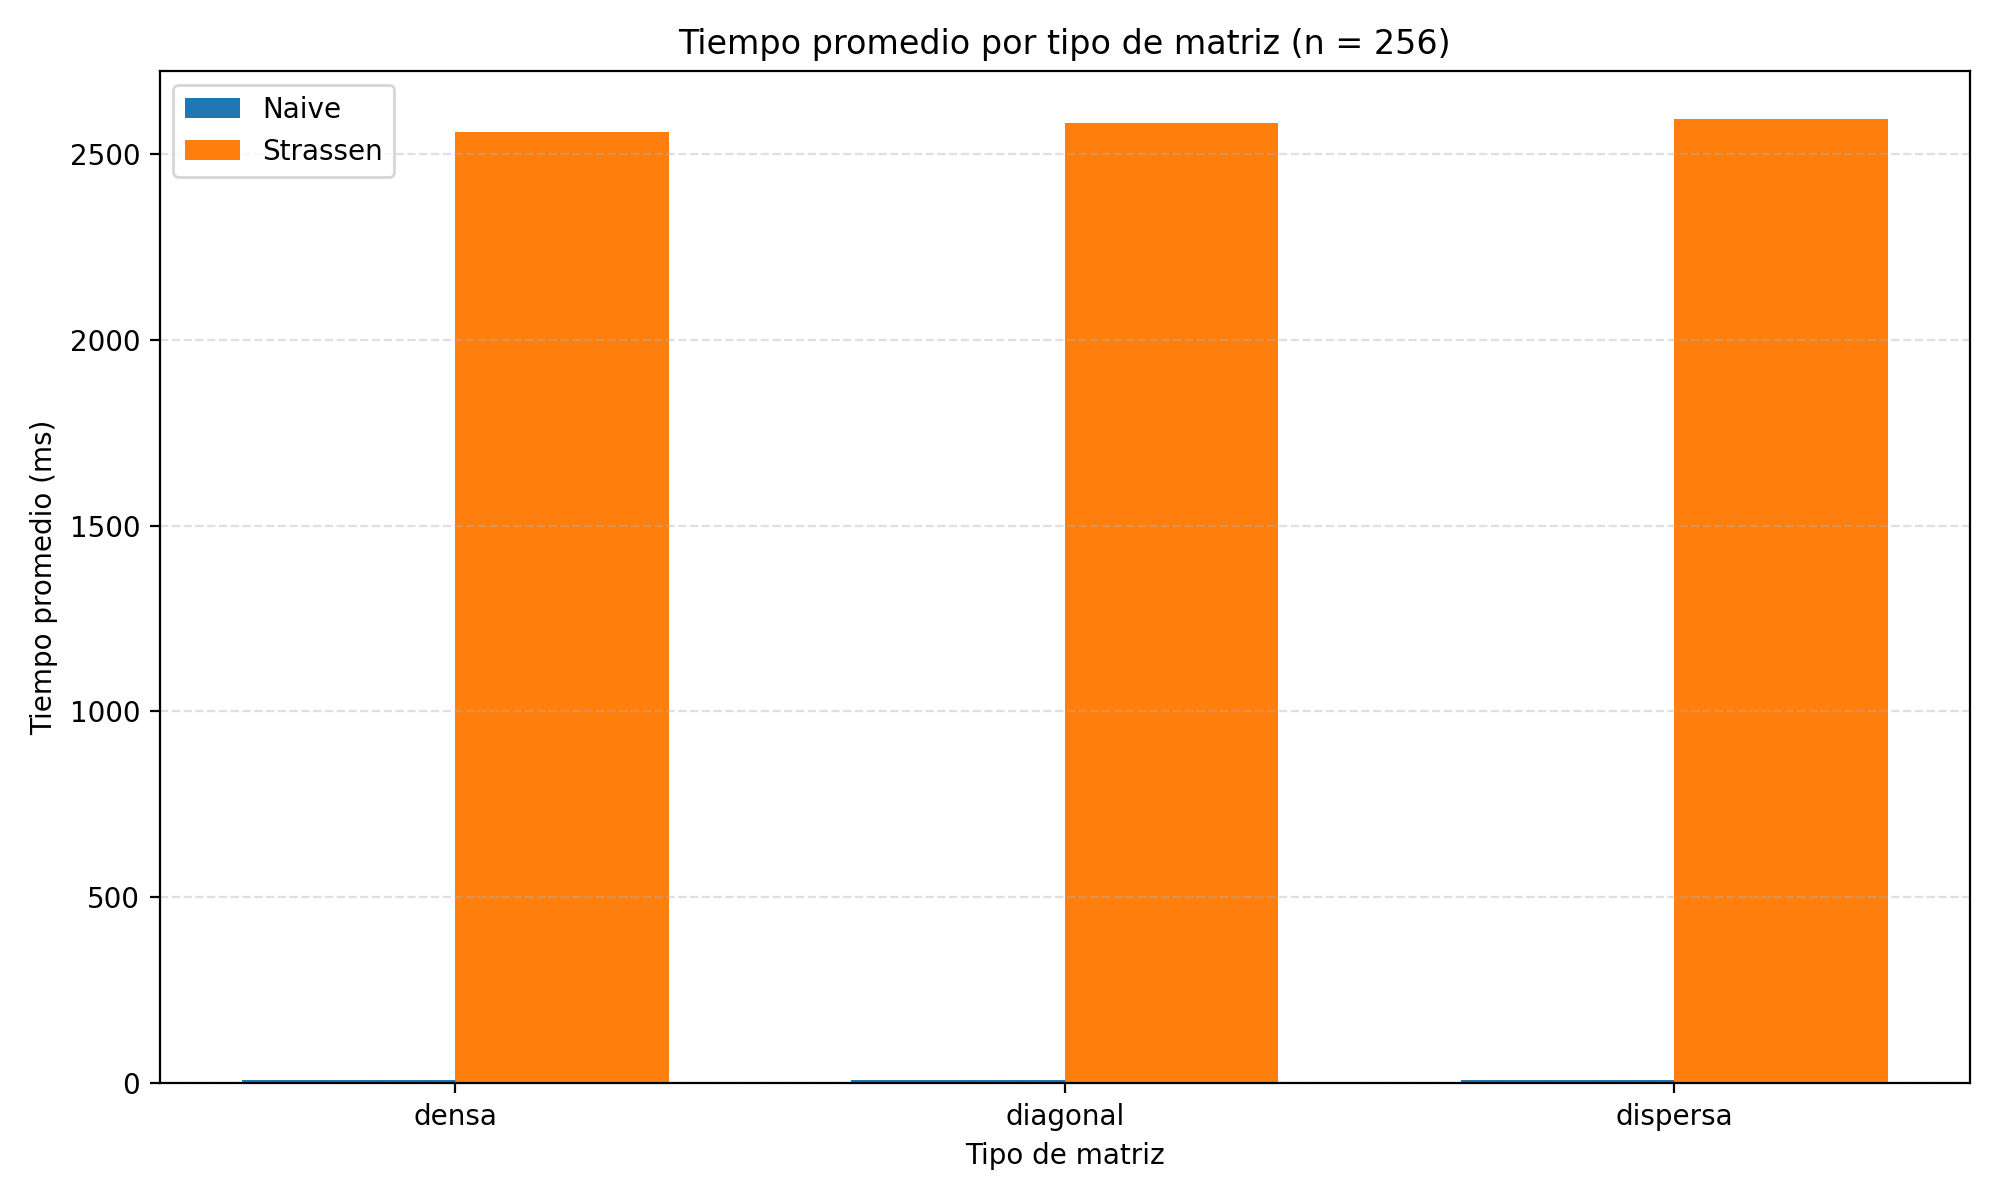
\includegraphics[width=\linewidth]{../code/matrix_multiplication/data/plots/matrix_barras_tiempo_n256.png}
                \caption{Tiempos}
                \label{fig:img12}
            \end{subfigure}

        \end{minipage}
    }
    \caption{Resultados para matrices 256x256}
    \label{fig:comparacion 256x256 matrix}
\end{figure}




\newpage
